\chapter{Introduction}\label{cha:intro}


\begin{figure}[!htb]
  \begin{center}
%% psfrag: comment the following line if not using the psfrag package
    % \psfrag{pie makes me happy!}{$\pi$ makes me happy!}
%% includegraphics: comment the following if not using the graphicx package
    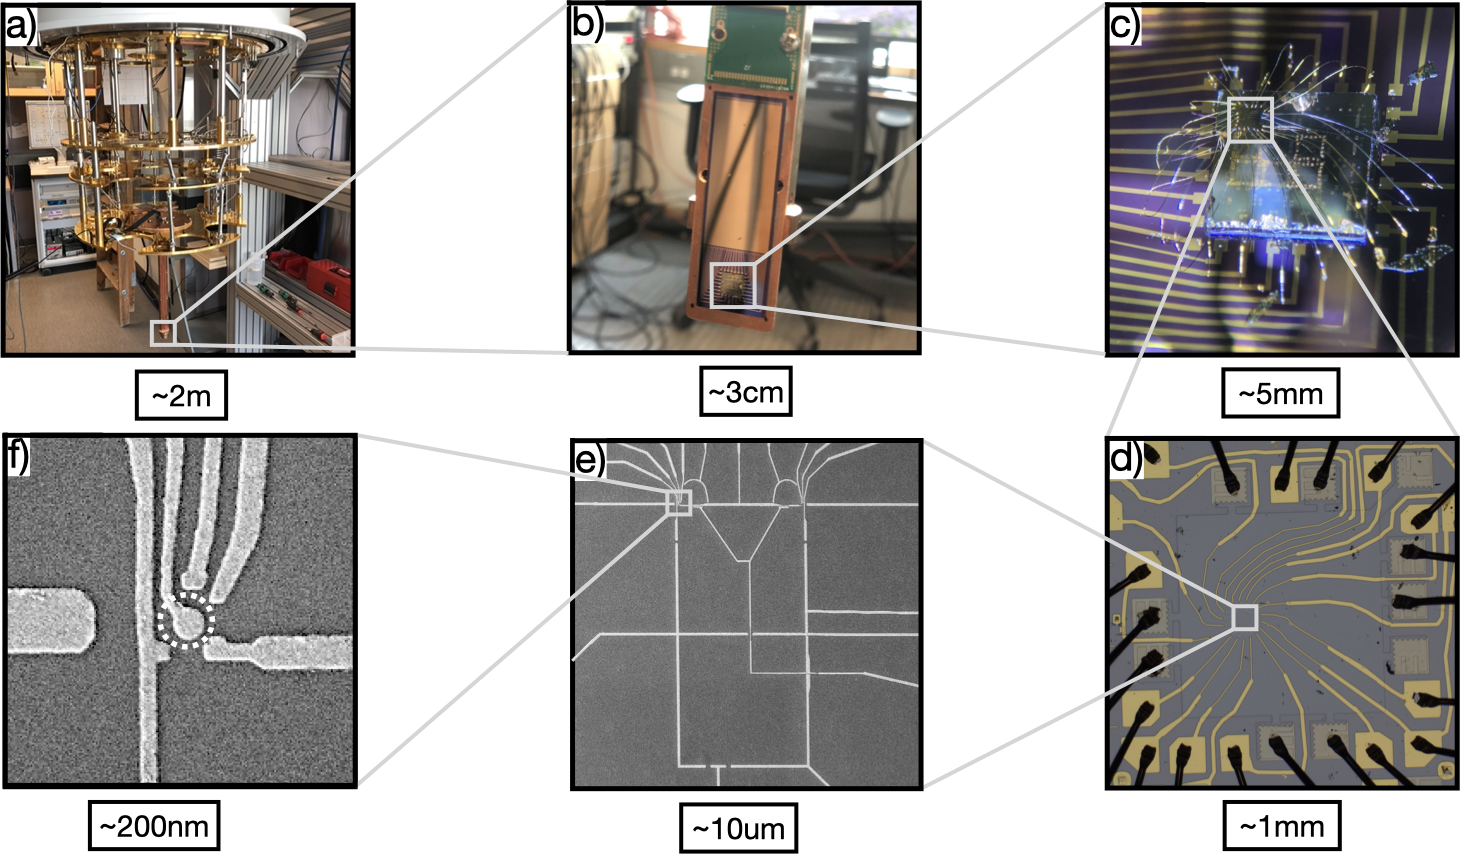
\includegraphics[width=1.0\textwidth]{figures/ch1/crop_PosterFiguresMaster.001.png}
    \caption[Dilution fridge to quantum dot scale breakdown]{\label{fig:ch1/scale_breakdown} 
    % For some options that work with pdf\LaTeX, please see this discussion:
    %   \url{http://tex.stackexchange.com/questions/11839}.  
    Showing the various scales to connect how macro changes affect the nano. (\textbf{a}) A photograph of the Au plated cold plates in our dilution refridgerator. The lowest plate is called the mixing chamber and can reach \qty{7}{mK}. (\textbf{b}) A photograph of the Si chip carrier, onto which the heterostructure is stuck to. (\textbf{c}) An optical microscope image of the heterostructure stuck to the chip carrier. The thin wires are Al wire bonds which connect the device fabricated on the heterostructure to the fridge wires. (\textbf{d}) An optical microscope image of a single mesa on the heterostructure. A mesa is an isolated area of the heterostructure where we fabricate new designs. The black lines around the outside are the wire bonds and the bright Au are the thick (\qty{100}{nm}) 'outer gates' which connect to the thin (\qty{10}{nm}) 'inner gates'. (\textbf{d}) A scanning electron micrograph (SEM) of the inner gates. The mean free path of the electrons is of order \qty{3}{\mu m}.  (\textbf{d}) An SEM image zoom-in on the quantum dot. By carefully tuning the voltages on the inner gates, we can create an isolated puddle of electrons, typically with total occupation 0 - 10.  
      }
  \end{center}
\end{figure}